% TU Delft Beamer template
% Author: Maarten Abbink
% Delft University of Technology
% March 2014
% Version 2.0
% Based on original version 1.0 of Carl Schneider
\documentclass{beamer}
\usepackage[english]{babel}
\usepackage{calc}
\usepackage[absolute,overlay]{textpos}
\usepackage{multicol}
\mode<presentation>{\usetheme{tud}}

\title[Beamer Sample]{Sample presentation using Beamer}
%\subtitle
\institute[TU Delft]{Delft University of Technology}
\author{Maarten Abbink}
\date{\today}

% Insert frame before each subsection (requires 2 latex runs)
\AtBeginSubsection[] {
	\begin{frame}<beamer>\frametitle{\titleSubsec}
	    \begin{multicols}{2}
		\tableofcontents[currentsection,currentsubsection]  % Generation of the Table of Contents
		\end{multicols}
	\end{frame}
}
% Define the title of each inserted pre-subsection frame
\newcommand*\titleSubsec{Next Subsection}
% Define the title of the "Table of Contents" frame
\newcommand*\titleTOC{Outline}

% define a symbol which can be removed if you don't need it
\newcommand{\field}[1]{\mathbb{#1}}
\newcommand{\Zset}{\field{Z}}

\begin{document}

{
% remove the next line if you don't want a background image
\usebackgroundtemplate{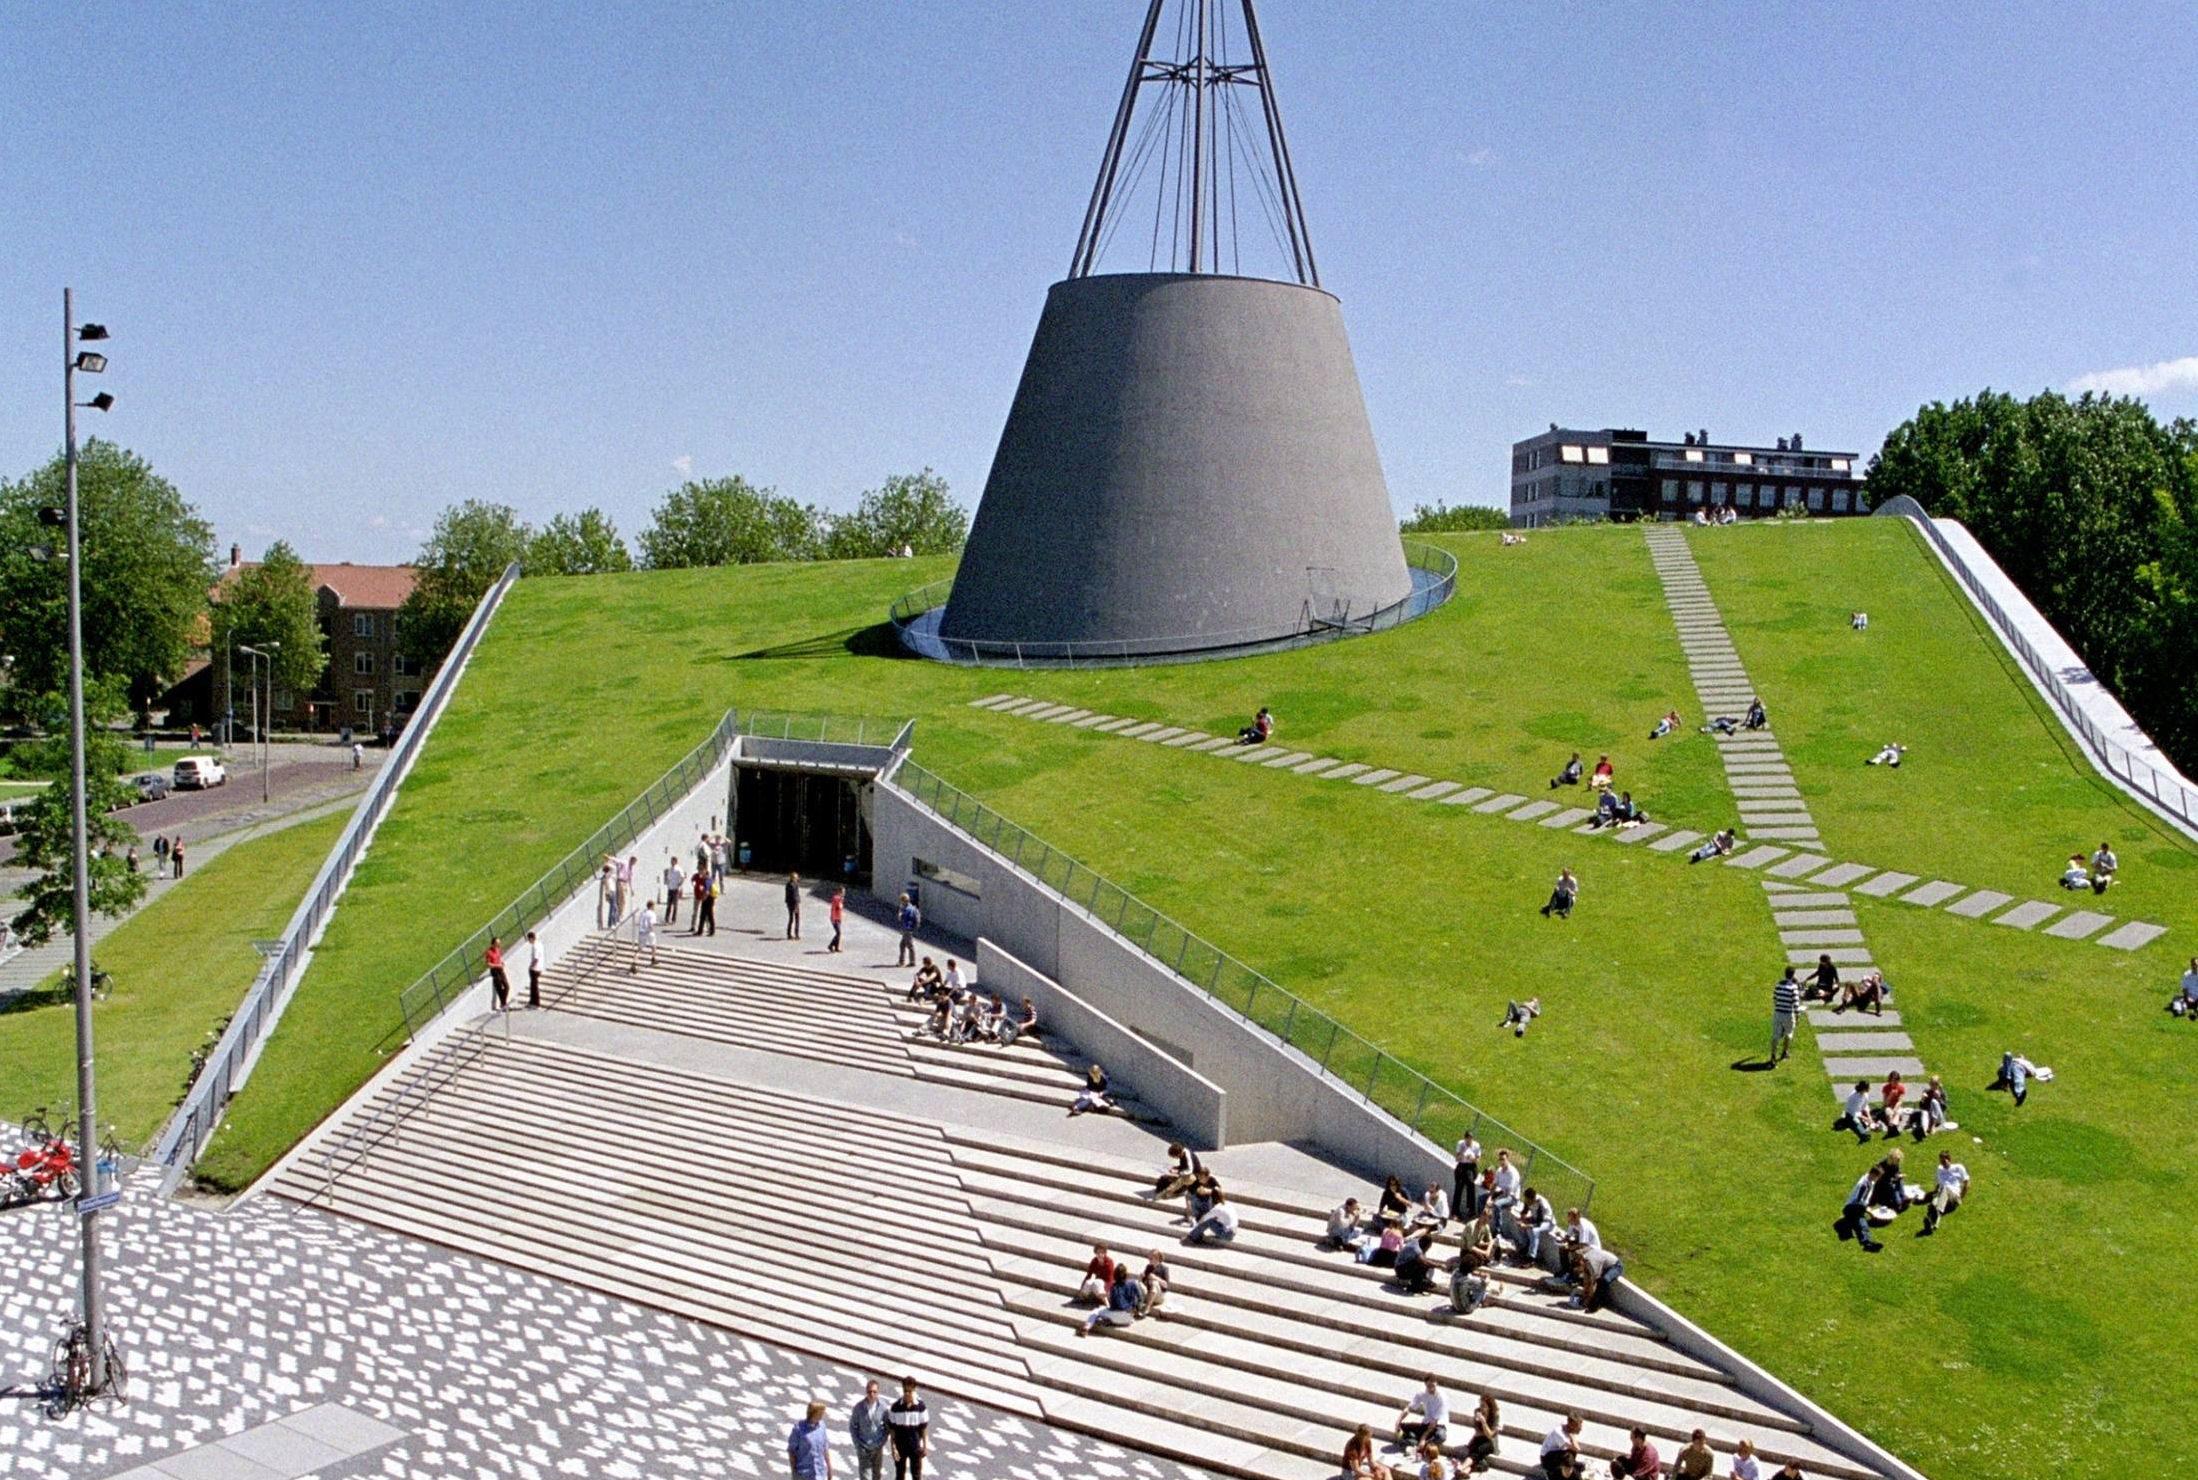
\includegraphics[width=\paperwidth,height=\paperheight]{images/background-titlepage.jpg}}%
\setbeamertemplate{footline}{\usebeamertemplate*{minimal footline}}
\frame{\titlepage}
}


{\setbeamertemplate{footline}{\usebeamertemplate*{minimal footline}}
\begin{frame}\frametitle{\titleTOC}
    \begin{multicols}{2}
	    \tableofcontents
	\end{multicols}
\end{frame}
}

\section{Introduction}

\subsection{Client}
\subsection{Motivation}
\subsection{Problem}

\begin{frame}\frametitle{Problem - Description}
    \begin{alertblock}{Problem}
		\centering{``How can the existing platform be extended in such a way that everyone in the FeedbackFruits community can contribute to the software development process?''}
	\end{alertblock}
	
\end{frame}

% The solution should bridge this gap in knowledge. Therefore, the contextual problem description can be defined as: “How can the existing platform be extended in such a way that everyone in the FeedbackFruits community can contribute to the software development process?”

\begin{frame}\frametitle{Problem - Analysis}
	\begin{enumerate}
        \item What can be learned from existing (non-software) communities?
        \item What current efforts exists to involve the community in the software development process?
        \item How are requirements established and used in software development?
        \item What limitations does the existing FeedbackFruits ecosystem impose on the software?
    \end{enumerate}
\end{frame}

% To anwser the four main research questions, the report will have four sections. The first research question zooms in on what can be learned from (non-software) communities. Before theories can be defined about what can be learned from all sorts of communities, a definition must be established of what a community is. Because communities exist in different sizes, with different structures and on different platforms, a few of these communities will be analysed in section 1.
% Some ways to involve the community in building software may be composed based on the previous section. However, this research will probably not be the only attempt to involve a software community in building software. The second research question is therefore focussed on existing platforms where software communities are involved in one way or another in the software development process. Section 2 will focus on the structure of the existing software communities. The techniques used by those communities and the way that the development process engages the community will also be examined.+

% Software development in its current form has some methodologies to establish requirements for a (big) software development project. The third research question will take a better look at the dynamics of requirements. These requirements are the basis of how the software will be built and are therefore an essential part of the software development process. In section 3, a few of the methods wich are used to establish requirements will be described. The dynamics of the requirements, like management and implementation, will also be given a closer look.
% The first three research question focus on determining the critical attributes of the problem in a general sense. However, because these attributes have to be applicable on the current FeedbackFruits-platform, that platform may pose some limitations. With research question four, the structure of the FeedbackFruits-platform will be examined, as well as the extensiblity of the platform. The result of this research question can be found in section 4.

% The most important aspects to this problem were identified in the research report as being: hype,requirements engineering, code and process updates (appendixD, chapter 5). Hype is necessary togain supporters that are willing to work on processing the feedback or feature requested by a user. Tobetter understand the how the feature should work, the feedback should be decomposed into smallchallenges via requirements engineering. These challenges should be converted to working code. Thecontributors should be informed of the current status of the feature through process updates. Thisprovides a feedback loop that ensures the challenges are tackled correctly.
\section{Research}

\subsection{Communities}
\begin{frame}\frametitle{Communities}
    \begin{enumerate}
        \item Goals
        \item Ideals
        \item Satisfaction
    \end{enumerate}
\end{frame}
\subsection{Software development}
\begin{frame}\frametitle{Software development}
    \begin{enumerate}
        \item Small core team
        \item Github or similar system
        \item Modular code
        \item Combined peer reviews and formal testing
        \item Stimulate intrinsic and extrinsic motivation
    \end{enumerate}
\end{frame}
\subsection{Requirements engineering}

\begin{frame}\frametitle{Requirements engineering}
    \begin{enumerate}
        \item Creating and managing requirements
        \item Decomposition into subproblems
        \item Iterative
    \end{enumerate}
\end{frame}
\subsection{FeedbackFruits ecosystem}
\begin{frame}\frametitle{FeedbackFruits ecosystem}
    \begin{enumerate}
        \item Architecture
        \item Software
        \item User experience
    \end{enumerate}
\end{frame}
\subsection{Conclusions}
\section{Solution}

\subsection{Design}
\begin{frame}\frametitle{Design}
	\begin{enumerate}
	    \item Implements FeedbackFruits' architecture
	    \item Goal-centered
	    \item Engagement via social media
	    \item Integration with GitHub for developers
	    \item Realtime communication
	\end{enumerate}
	
% 	Plaatje Goals<-Supporters<-Social media <- GitHub
\end{frame}

\subsection{Challenges}
\begin{frame}\frametitle{Challenges}
	\begin{enumerate}
	    \item Planning
	    \item API standards
	    \item Shared codebase
	    \item Experimental web-technologies
	\end{enumerate}
	
% 	Plaatje Goals<-Supporters<-Social media <- GitHub
\end{frame}

\subsection{Demo}
\begin{frame}\frametitle{Demo}
\begin{alertblock}{Demo}
		\centering{\Large{Demo}}
	\end{alertblock}
\end{frame}
\subsection{Results}
\section{Conclusion}

\begin{frame}\frametitle{What was the problem again}
    \begin{alertblock}{Problem}
		\centering{``How can the existing platform be extended in such a way that everyone in the FeedbackFruits community can contribute to the software development process?''}
	\end{alertblock}
\end{frame}

\subsection{What was accomplished}
\subsection{Improvements}
\begin{frame}\frametitle{Improvements}
    \begin{enumerate}
        \item Planning
        \item More communication options
        \item Hype measurement
        \item Design contributions
        \item Contribution feedback
        \item Templates
    \end{enumerate}
\end{frame}
\subsection{Verification}

\begin{frame}\frametitle{Verification}
    \begin{figure}[ht!]
        \centering
        
\includegraphics[width=0.8\textwidth]{./media/hackathon-graphic}
        \caption{by Clarus Commerce}
        \label{fig:goal-design}
    \end{figure}
\end{frame}

% Include line below to see a sample
% \section{First Section}
\subsection{Section 1 - Subsection 1}

\begin{frame}\frametitle{Section 1 - Subsection 1 - Page 1}
	\begin{example}
		\begin{minipage}{0.6\textwidth}
			% insert picture (pdf file)
			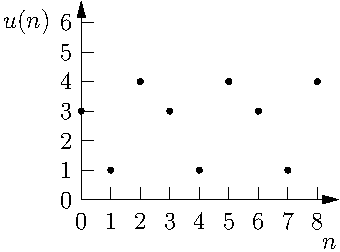
\includegraphics{images/ex1_periodic_number.pdf}
		\end{minipage}
		\centering{$u(n)=[3,1,4]_n$}
	\end{example}
\end{frame}

\begin{frame}\frametitle{Section 1 - Subsection 1 - Page 2}
	\begin{definition}
		Let $n$ be a discrete variable, i.e. $n\in\Zset$.
		A 1-dimensional periodic number is a function that depends periodically on $n$.
		$$
		u(n)=
		[u_0,u_1,\ldots,u_{d-1}]_n=
		\begin{cases}
			u_0 & \mbox{ if $n\equiv 0 \pmod d$} \\
			u_1 & \mbox{ if $n\equiv 1 \pmod d$} \\
			\vdots \\
			u_{d-1} & \mbox{ if $n\equiv d-1 \pmod d$}
		\end{cases}
		$$
		$d$ is called the period.
	\end{definition}
\end{frame}

\begin{frame}\frametitle{Section 1 - Subsection 1 - Page 3}
	%this is too big.
	\begin{example}
		\centering
		{
		$$
		\begin{array}{rcl}
			f(n)
			&=&
			-\left[\frac{1}{2},\frac{1}{3}\right]_n n^2
			+3n-[1,2]_n
			\\
			&=&
			\begin{cases}
				-\frac{1}{3} n^2 +3n-2
				& \text{ if $n\equiv 0 \pmod 2$} \\
				-\frac{1}{2} n^2 +3n-1
				& \text{ if $n\equiv 1 \pmod 2$}
			\end{cases}
			% &=&
			% -\frac{n^2}{2}+3n-1
			% -\left\{ \frac{n}{2} \right\}
			% \left( \frac{2}{3}n^2+2
			% \right)
		\end{array}
		$$
		\begin{minipage}{0.4\textwidth}
			% insert picture (pdf file)
			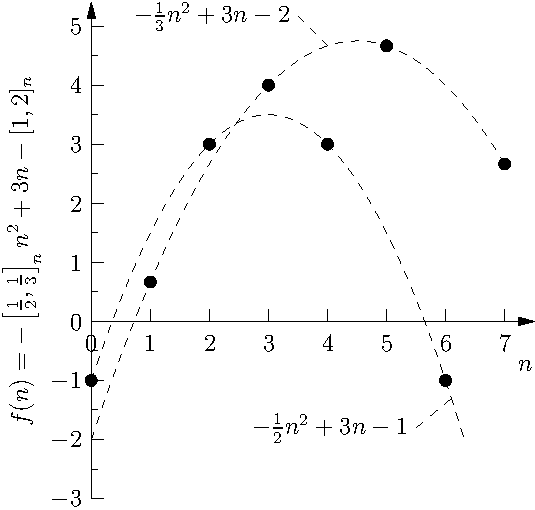
\includegraphics[width=\textwidth]{images/ex2_quasi_polynomial.pdf}
		\end{minipage}
		}
	\end{example}
\end{frame}

\begin{frame}\frametitle{Section 1 - Subsection 1 - Page 4}
	% Show first part of the screen highlighted
	\begin{definition}
		A polynomial in a variable $x$ is a linear combination of powers of $x$:
		$$
		f(x)=\sum_{i=0}^g c_i x^i
		$$
	\end{definition}
	\pause
	
	% Show second part of the screen highlighted
	\begin{definition}
		A quasi-polynomial in a variable $x$ is a polynomial expression with periodic numbers as coefficients:
		$$
		f(n)=\sum_{i=0}^g u_i(n) n^i
		$$
		with $u_i(n)$ periodic numbers.
	\end{definition}
\end{frame}

\subsection{Section 1 - Subsection 2}

\begin{frame}\frametitle{Section 1 - Subsection 2 - Page 1}
	\begin{example}
		\begin{columns}
			\column{0.40\textwidth}
			\centering
			\includegraphics<1>[width=\textwidth]{images/ex3a_pp.pdf}
			\includegraphics<2>[width=\textwidth]{images/ex3b_pp.pdf}
			\includegraphics<3>[width=\textwidth]{images/ex3c_pp.pdf}
			\includegraphics<4->[width=\textwidth]{images/ex3d_pp.pdf}
			{ \textbf{\small{{$x+y\le p$}}}}
			\column{0.1\textwidth}
			
			\begin{tabular}{c c}
				$p$ & $f(p)$ \\ \hline
				3 & 5 \\
				\pause
				4 & 8 \\
				\pause
				5 & 10 \\
				\pause
				6 & 13 \\
			\end{tabular}
			
			\column{0.3\textwidth}
			\pause
			$$
			\frac{5}{2}p+\left[-2,\frac{-5}{2} \right]_p
			$$
		\end{columns}
	\end{example}
\end{frame}

\begin{frame}\frametitle{Section 1 - Subsection 2 - Page 2}
	\begin{itemize}
		\item <1-> The number of integer points in a \alert{parametric polytope} $P_{{p}}$ of dimension $n$ is expressed as a piecewise a quasi-polynomial of degree $n$ in ${p}$ (Clauss and Loechner).
		
		\item <2->
		More general \alert{polyhedral counting problems}:\\
		Systems of linear inequalities combined with $\lor, \land, \neg, \forall,$ or $\exists$ (Presburger formulas).
		\item <3->
		Many problems in \alert{static program analysis} can be expressed as polyhedral counting problems.
	\end{itemize}
\end{frame}

\subsection{Section 1 - Subsection 3}

\begin{frame}\frametitle{Section 1 - Subsection 3 - Page 1}
	% Just an example
	A picture made with the package TiKz\\
	\begin{example}
		\centering
		%Number of live elements = quasi-polynomial\\
		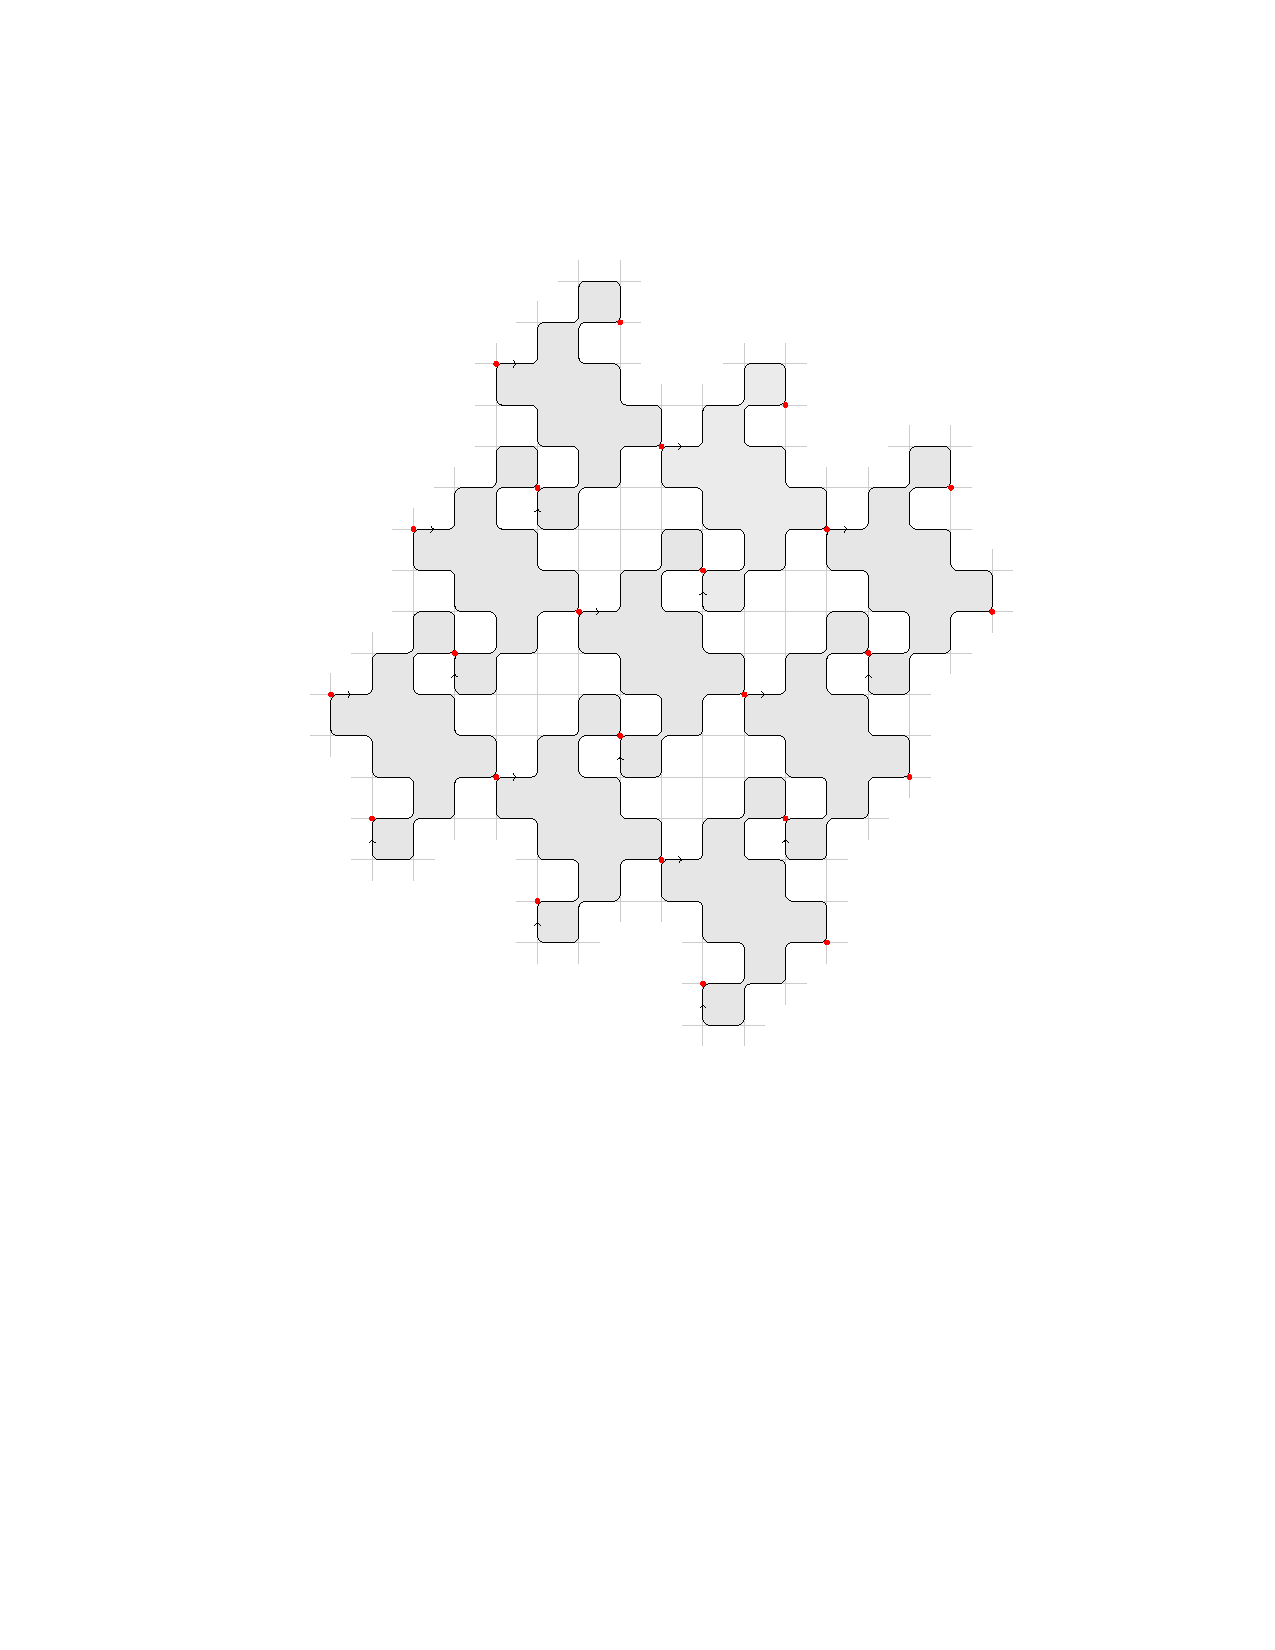
\includegraphics[width=5cm]{images/abadab-anti-theta-01.pdf}
		%$\Downarrow$ \\
		%Memory usage = maximum over all execution points
	\end{example}
\end{frame}

\section{Second Section}

\subsection{Section 2 - Subsection 1}

\begin{frame}\frametitle{Section 2 - subsection 1 - page 1}
	\begin{alertblock}{Alertblock}
		This page gives an example with numbered bullets (enumerate)\\
		in an "Example" window:\\
	\end{alertblock}
	
	\begin{example}
		Discrete domain $\Rightarrow$ evaluate in each point\\
		Not possible for\\
		\begin{enumerate}
			\item <1-> parametric domains
			\item <2-> large domains (NP-complete)
		\end{enumerate}
	\end{example}
\end{frame}

\subsection[]{Section 2 - Last Subsection}

\begin{frame}\frametitle{Last Page}
	\begin{block}{Summary}
		\centering{End of the beamer demo\\
		with a \emph{tidy} TU~Delft lay-out.\\
		Thank you!}
	\end{block}
\end{frame}


\end{document}
